\chapter{Experimental Evaluation}

This chapter presents the results of the four experimental scenarios designed to answer the three research questions. Each experiment is described in terms of its setup, the results obtained, and a brief interpretation.

\section{Experimental Setup}

All BERT experiments follow the pipeline and hyperparameter configuration described in Section~4.1. The base model is BERT\textsubscript{BASE-UNCASED} with the six-category multi-label head, trained with the Adam optimiser at a learning rate of $3\times10^{-5}$, a batch size of 16, a maximum sequence length of 300 tokens, and a binary decision threshold of 0.20. Training runs for up to five epochs on an NVIDIA T4 GPU (Google Colaboratory), with early stopping on the validation loss and retention of the checkpoint achieving the lowest validation loss (Section~4.1).

To account for training stochasticity, each experimental condition is repeated over ten seeds. For every seed the corresponding dataset is partitioned into training (85\%) and validation (15\%) subsets using that seed's random state, the model is trained from scratch, and its performance is evaluated on the held-out validation partition. Reported metrics are those of the best retained checkpoint of each seed, averaged over the ten runs; the mean and standard deviation across seeds are reported. Because all conditions share this identical protocol, any observed differences reflect the data, not the training procedure.

\section{Baseline: BERT on the Full Dataset}

The baseline condition trains and evaluates BERT on the full 2,166-sentence dataset (Section~\ref{sec:exp-design}), reproducing the AI-CRAS configuration as closely as the available data permits. It establishes the reference performance against which the ambiguity-related conditions are compared.

On the binary requirement-detection task, the baseline achieves a precision of 0.816, a recall of 0.942, and an F1-score of 0.874. The large gap between recall and precision reflects the chosen operating point (threshold 0.20, Section~4.1), which favours identifying requirements over avoiding false positives: the model rarely misses a requirement, but over-assigns the label to some non-requirement sentences.

On the multi-label task, the baseline attains a macro-averaged F1 of 0.675 (macro precision 0.591, macro recall 0.809), a micro-averaged F1 of 0.676, and an exact-match accuracy of 0.516, with a Hamming loss of 0.115 and a Jaccard score of 0.514. As on the binary task, macro recall markedly exceeds macro precision across all six categories, the same systematic over-prediction pattern later observed for the LLM classifiers in Section~5.5.

Table~\ref{tab:bert_perlabel} reports the per-category F1-scores for the baseline and, for reference, the two experimental conditions described in the following sections. Security \& Compliance is classified most reliably (0.748), followed by Network (0.724) and Management \& Monitoring (0.673); Compute (0.611), Data Handling (0.652), and Cloud Service Essentials (0.642) are the hardest. The comparatively weak performance on the latter three is consistent with the difficulty these categories pose in the raw data.

\begin{table}[h]
\centering
\caption{F1-scores by cloud service category for the three BERT conditions (mean $\pm$ std over ten seeds).}
\label{tab:bert_perlabel}
\footnotesize
\begin{tabular}{lccc}
\toprule
Category & Baseline & No-ambiguity & Deambiguified \\
\midrule
Compute                    & $0.611 \pm 0.045$ & $0.594 \pm 0.063$ & $0.598 \pm 0.072$ \\
Data Handling              & $0.652 \pm 0.080$ & $0.594 \pm 0.070$ & $0.643 \pm 0.065$ \\
Network                    & $0.724 \pm 0.070$ & $0.729 \pm 0.089$ & $0.718 \pm 0.064$ \\
Security \& Compliance     & $0.748 \pm 0.037$ & $0.751 \pm 0.041$ & $0.749 \pm 0.049$ \\
Management \& Monitoring   & $0.673 \pm 0.037$ & $0.697 \pm 0.053$ & $0.679 \pm 0.040$ \\
Cloud Service Essentials   & $0.642 \pm 0.089$ & $0.635 \pm 0.066$ & $0.651 \pm 0.077$ \\
\bottomrule
\end{tabular}
\end{table}

\section{RQ1 --- Effect of Ambiguity on BERT Classification}

To test whether ambiguity degrades classification performance, BERT was trained and evaluated exclusively on the 1,854 unambiguous sentences (the no-ambiguity subset of Section~\ref{sec:exp-design}), and the outcome was compared against the full-dataset baseline.

The results are statistically indistinguishable from the baseline. Removing the 312 sentences judged ambiguous changes the macro-averaged F1 from 0.675 (baseline) to 0.667 (no-ambiguity)---a difference of 0.008 that is far smaller than the run-to-run variability (standard deviations of 0.026 and 0.038, respectively). The binary requirement F1 is likewise essentially unchanged (0.871 \textit{vs.}~0.874), as is the exact-match accuracy (0.528 \textit{vs.}~0.516). At the category level (Table~\ref{tab:bert_perlabel}), no category changes by more than about 0.06, and the shifts show no consistent direction: Management \& Monitoring improves slightly, while Compute and Data Handling decline slightly.

These results do not support the hypothesis that ambiguity, as annotated, degrades BERT-based requirement classification. Filtering out the ambiguous sentences yields a smaller training set whose performance matches the full dataset within noise, rather than a cleaner set that performs better. The interpretation of this null finding---and its relation to the subjectivity of ambiguity annotation documented in Section~3.2---is discussed in Chapter~6.

\section{RQ2 --- BERT on LLM-Disambiguated Sentences}

To test whether rewriting ambiguous sentences into clearer versions improves classification, BERT was trained and evaluated on the deambiguified dataset (Section~\ref{sec:exp-design}), in which every sentence judged ambiguous is replaced by its LLM-rewritten counterpart while unambiguous sentences are kept verbatim.

As with RQ1, the results are indistinguishable from the baseline. The deambiguified condition attains a macro-averaged F1 of 0.673 (\textit{vs.}~0.675 for the baseline), a binary requirement F1 of 0.871 (\textit{vs.}~0.874), and an exact-match accuracy of 0.517 (\textit{vs.}~0.516). Every aggregate metric lies within one standard deviation of its baseline counterpart. At the category level (Table~\ref{tab:bert_perlabel}) no category changes by more than about 0.015, and Cloud Service Essentials---the category with the highest ambiguity rate (Section~3.3)---shows the largest, still negligible, improvement.

Substituting clearer formulations of ambiguous sentences therefore neither helps nor hurts: classification performance on the rewritten corpus is effectively identical to that on the original one. This null result is consistent with the finding of Section~5.3: if ambiguity does not measurably impair the classifier to begin with, there is little room for disambiguation to improve it. The implications are discussed in Chapter~6.

\section{RQ3 --- LLM as Direct Classifier}

This section evaluates GPT\textsubscript{4.1-mini} and GPT\textsubscript{5.4-mini} as standalone classifiers in zero-shot and few-shot configurations. All experiments use temperature 0, the category definitions from Section~4.3.1, and the batch-processing protocol described in Section~4.3. Following the AI-CRAS evaluation protocol~\cite{casalicchio2024aicras}, binary classification is reported as per-class P/R/F1 and multi-label classification as per-category and macro-averaged P/R/F1.

\subsection{Zero-Shot Results}

Table~\ref{tab:rq3_zeroshot} reports the binary classification and Table~\ref{tab:rq3_zeroshot_perlabel} the per-category breakdown on 2,166 sentences.

\begin{table}[h]
\centering
\caption{Zero-shot binary classification results on the full dataset (2,166 sentences).}
\label{tab:rq3_zeroshot}
\begin{tabular}{lccc}
\toprule
Class & Precision & Recall & F1 \\
\midrule
\multicolumn{4}{c}{\textit{GPT\textsubscript{4.1-mini}}} \\
\midrule
Non-Requirement & 0.772 & 0.465 & 0.580 \\
Requirement     & 0.789 & 0.936 & 0.856 \\
\midrule
\multicolumn{4}{c}{\textit{GPT\textsubscript{5.4-mini}}} \\
\midrule
Non-Requirement & 0.732 & 0.376 & 0.497 \\
Requirement     & 0.762 & 0.936 & 0.840 \\
\bottomrule
\end{tabular}
\end{table}

Both models achieve high Recall on the Requirement class (0.936). GPT\textsubscript{4.1-mini} yields marginally higher F1-scores across both classes, with the gap most pronounced on Non-Requirement detection (F1 0.580 \textit{vs.} 0.497).

Table~\ref{tab:rq3_zeroshot_perlabel} breaks down performance by cloud service category.

\begin{table}[h]
\centering
\caption{Per-label zero-shot classification results.}
\label{tab:rq3_zeroshot_perlabel}
\footnotesize
\begin{tabular}{lcccccc}
\toprule
& \multicolumn{3}{c}{GPT\textsubscript{4.1-mini}} & \multicolumn{3}{c}{GPT\textsubscript{5.4-mini}} \\
\cmidrule(lr){2-4} \cmidrule(lr){5-7}
Category & P & R & F1 & P & R & F1 \\
\midrule
Compute                       & 0.423 & 0.738 & 0.538 & 0.423 & 0.694 & 0.525 \\
Data Handling                 & 0.375 & 0.879 & 0.525 & 0.364 & 0.885 & 0.516 \\
Network                       & 0.538 & 0.867 & 0.664 & 0.561 & 0.849 & 0.675 \\
Security \& Compliance         & 0.565 & 0.907 & 0.696 & 0.599 & 0.869 & 0.709 \\
Management \& Monitoring       & 0.651 & 0.541 & 0.591 & 0.642 & 0.591 & 0.616 \\
Cloud Service Essentials      & 0.402 & 0.411 & 0.406 & 0.374 & 0.431 & 0.401 \\
\midrule
Macro Average                 & 0.492 & 0.724 & 0.570 & 0.494 & 0.720 & 0.574 \\
\bottomrule
\end{tabular}
\end{table}

Performance varies considerably across categories. Security \& Compliance is the strongest (F1 0.696--0.709) and Cloud Service Essentials the weakest (0.401--0.406). Recall uniformly exceeds precision across all categories and both models, a systematic over-prediction pattern explored further in the few-shot results.

\subsection{Few-Shot Results}

In the few-shot setting, 16 distribution-matched demonstrations (Section~4.3.3) are prepended to the prompt. Table~\ref{tab:rq3_fewshot} reports the per-class binary performance and Table~\ref{tab:rq3_fewshot_perlabel} the per-category breakdown.

\begin{table}[h]
\centering
\caption{Few-shot binary classification results on 1,966 sentences (200 held out as example pool).}
\label{tab:rq3_fewshot}
\begin{tabular}{lccc}
\toprule
Class & Precision & Recall & F1 \\
\midrule
\multicolumn{4}{c}{\textit{GPT\textsubscript{4.1-mini}}} \\
\midrule
Non-Requirement & 0.700 & 0.516 & 0.594 \\
Requirement     & 0.792 & 0.893 & 0.840 \\
\midrule
\multicolumn{4}{c}{\textit{GPT\textsubscript{5.4-mini}}} \\
\midrule
Non-Requirement & 0.744 & 0.317 & 0.444 \\
Requirement     & 0.741 & 0.947 & 0.832 \\
\bottomrule
\end{tabular}
\end{table}

\begin{table}[h]
\centering
\caption{Per-label few-shot classification results.}
\label{tab:rq3_fewshot_perlabel}
\footnotesize
\begin{tabular}{lcccccc}
\toprule
& \multicolumn{3}{c}{GPT\textsubscript{4.1-mini}} & \multicolumn{3}{c}{GPT\textsubscript{5.4-mini}} \\
\cmidrule(lr){2-4} \cmidrule(lr){5-7}
Category & P & R & F1 & P & R & F1 \\
\midrule
Compute                       & 0.472 & 0.699 & 0.563 & 0.478 & 0.673 & 0.559 \\
Data Handling                 & 0.410 & 0.873 & 0.558 & 0.382 & 0.836 & 0.525 \\
Network                       & 0.600 & 0.796 & 0.684 & 0.566 & 0.806 & 0.665 \\
Security \& Compliance         & 0.581 & 0.813 & 0.678 & 0.607 & 0.828 & 0.700 \\
Management \& Monitoring       & 0.695 & 0.531 & 0.602 & 0.551 & 0.659 & 0.600 \\
Cloud Service Essentials      & 0.319 & 0.138 & 0.193 & 0.346 & 0.377 & 0.361 \\
\midrule
Macro Average                 & 0.513 & 0.642 & 0.546 & 0.488 & 0.696 & 0.568 \\
\bottomrule
\end{tabular}
\end{table}

GPT\textsubscript{4.1-mini} achieves stronger binary performance, particularly on Non-Requirement recall (0.516 \textit{vs.} 0.317), indicating less over-prediction. On the multi-label task, however, GPT\textsubscript{5.4-mini} leads on macro F1 (0.568 \textit{vs.} 0.546), largely because GPT\textsubscript{4.1-mini} severely underpredicts Cloud Service Essentials (recall 0.138, F1 0.193). For neither model does the few-shot configuration improve over zero-shot. The implications are discussed in Chapter~6.

\section{Cross-Experiment Comparison}
\label{sec:cross-experiment}

Table~\ref{tab:cross_experiment} consolidates the binary Requirement-class and macro-averaged multi-label metrics for all experimental conditions: the three BERT conditions of this thesis, the four LLM conditions, and the original AI-CRAS BERT~\cite{casalicchio2024aicras} reproduced as a reference. To make the comparison meaningful, the BERT figures are the mean over the ten seeds of the best retained checkpoint, and the LLM figures are computed on the same 2,166-sentence evaluation population.

\begin{table}[h]
\centering
\caption{Binary Requirement-class and macro-averaged multi-label results for the BERT and LLM conditions. AI-CRAS figures are reproduced from~\cite{casalicchio2024aicras}.}
\label{tab:cross_experiment}
\footnotesize
\begin{tabular}{lcccccc}
\toprule
Condition & Req P & Req R & Req F1 & Macro P & Macro R & Macro F1 \\
\midrule
\multicolumn{7}{l}{\textit{Fine-tuned BERT (this thesis, mean over 10 seeds)}} \\
\midrule
Baseline              & 0.816 & 0.942 & 0.874 & 0.591 & 0.809 & 0.675 \\
No-ambiguity (RQ1)    & 0.812 & 0.945 & 0.871 & 0.586 & 0.801 & 0.667 \\
Deambiguified (RQ2)   & 0.809 & 0.944 & 0.871 & 0.597 & 0.791 & 0.673 \\
\midrule
AI-CRAS BERT~\cite{casalicchio2024aicras}      & 0.88 & 0.96 & 0.92 & 0.70 & 0.86 & 0.76 \\
\midrule
\multicolumn{7}{l}{\textit{LLM as direct classifier (this thesis)}} \\
\midrule
LLM Zero-Shot GPT\textsubscript{4.1-mini}       & 0.789 & 0.936 & 0.856 & 0.492 & 0.724 & 0.570 \\
LLM Zero-Shot GPT\textsubscript{5.4-mini}       & 0.762 & 0.936 & 0.840 & 0.494 & 0.720 & 0.574 \\
LLM Few-Shot GPT\textsubscript{4.1-mini}       & 0.792 & 0.893 & 0.840 & 0.513 & 0.642 & 0.546 \\
LLM Few-Shot GPT\textsubscript{5.4-mini}       & 0.741 & 0.947 & 0.832 & 0.488 & 0.697 & 0.568 \\
\bottomrule
\end{tabular}
\end{table}

Figure~\ref{fig:cross_experiment} visualises these comparisons, and Table~\ref{tab:cross_experiment} reports the underlying values; error bars on the BERT conditions indicate the standard deviation over the ten seeds.

\begin{figure}[h]
\centering
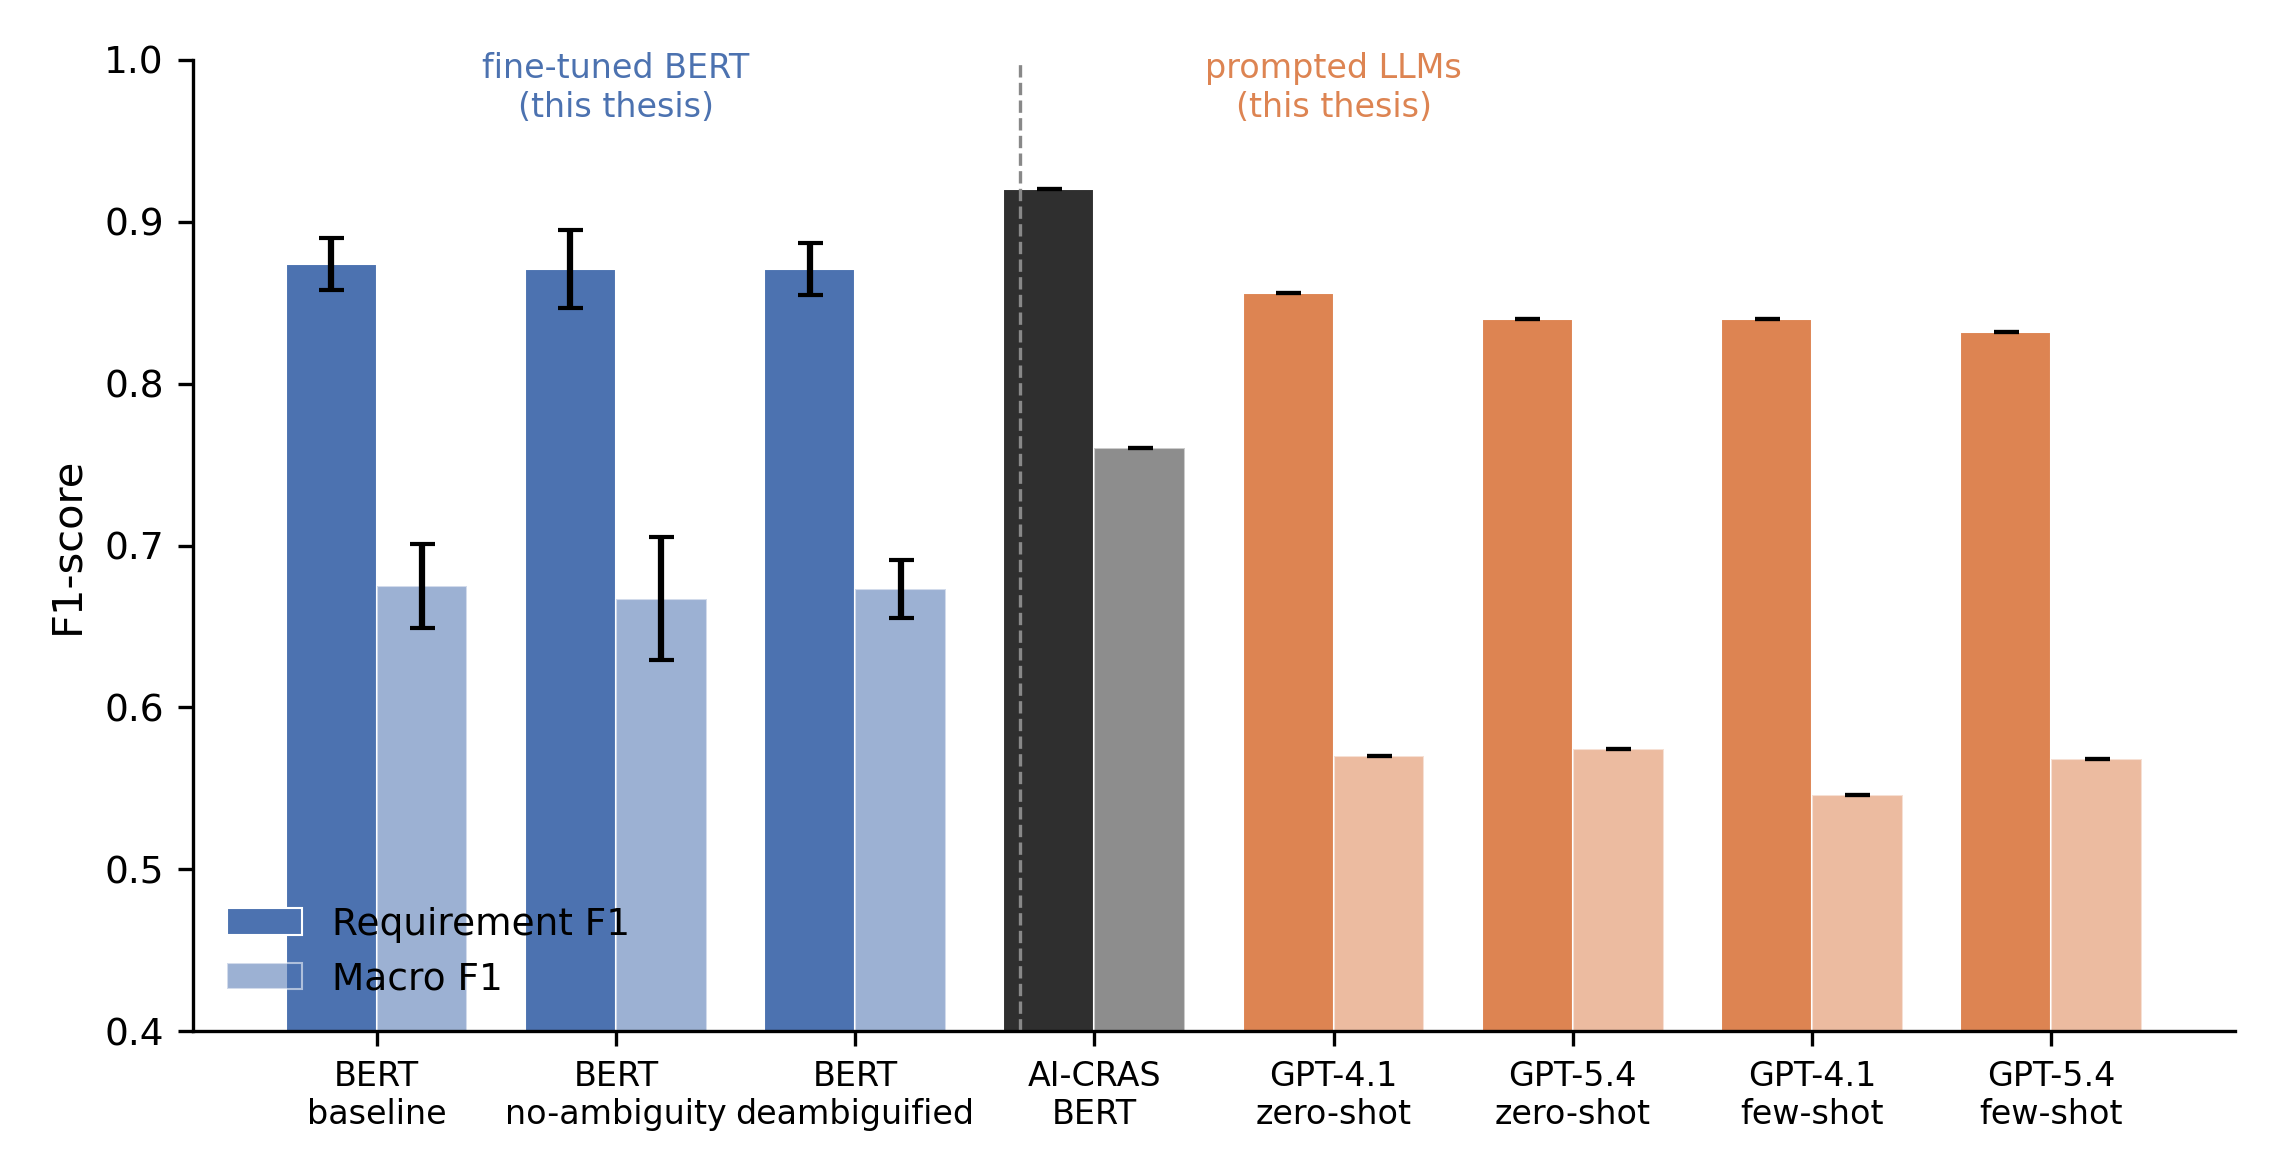
\includegraphics[width=0.9\textwidth]{figures/fig5_cross_experiment.png}
\caption{Requirement-class and macro-averaged F1 across conditions. Error bars on the fine-tuned BERT conditions show the standard deviation over the ten seeds; the dashed line separates the reproduced BERT conditions from the reference and the prompted-LLM conditions.}
\label{fig:cross_experiment}
\end{figure}

The three BERT conditions of this thesis perform essentially identically (binary requirement F1 of 0.871--0.874 and macro F1 of 0.667--0.675), confirming that the ambiguity manipulations of RQ1 and RQ2 have no measurable effect. The reproduced baseline falls somewhat below the original AI-CRAS BERT (binary F1 0.874 \textit{vs.}~0.92; macro F1 0.675 \textit{vs.}~0.76); the origin of this gap, which includes differences in the evaluation protocol, is examined in Chapter~6.

All LLM conditions fall below the fine-tuned BERT baseline of this thesis on both tasks. On binary Requirement detection, the best LLM reaches a requirement F1 of 0.856, close to---but below---the BERT baseline's 0.874, with a similar profile of high recall (0.936) and lower precision. On the multi-label task the gap is larger: the LLMs reach a macro F1 of 0.546--0.574, well below the BERT baseline's 0.675. General-purpose prompting therefore does not match a domain fine-tuned model, despite the LLMs' strong recall.

Among the LLMs, the two models perform near-identically in zero-shot. Few-shot demonstrations do not yield consistent improvement: GPT\textsubscript{5.4-mini} is nearly flat (macro F1 0.568 \textit{vs.}~0.574), while GPT\textsubscript{4.1-mini} improves binary detection but collapses on Cloud Service Essentials (F1 0.193, see Table~\ref{tab:rq3_fewshot_perlabel}), producing the lowest macro F1 of any configuration (0.546). This reinforces the finding that category descriptions alone carry sufficient signal, and that in-context examples may introduce distributional bias---a point discussed further in Chapter~6.
